A valid question is the effect on the limits on each Higgs mass hypothesis in
the case of the presence of a Higgs signal at a given mass. As a test, we
consider a Higgs with $\mHi = 125~\GeV$, and see the effect on the limits, both
cut-based and BDT-based analyses. The expected and observed upper 
limits are reported in Tables~\ref{tab:cutbased_mh125_nj} 
and~\ref{tab:bdtbased_mh125_nj}, and 
in Figure~\ref{fig:uls_mh125_nj}. The observed upper limits in this context are 
the mean average limits in the presence of background plus signal.

%%%%%%%%%%%%%%%%%%%%%%%%%%%%%%
\begin{table}[hbp!]
\begin{center}
\begin{tabular}{c c c c c}
\hline
\vspace{-3mm} && \\
 Higgs Mass & Pseudo-data  & Median expected & Expected range for 68\% & Expected range for 95\%   \\
\vspace{-3mm} && \\
\hline
110 & 10.79 & 5.93 & [4.27, 8.25] & [3.18, 11.06] \\
115 & 5.43 & 3.20 & [2.31, 4.45] & [1.72, 5.97] \\
120 & 3.36 & 1.91 & [1.37, 2.65] & [1.02, 3.56] \\
125 & 2.18 & 1.29 & [0.93, 1.80] & [0.69, 2.41] \\
130 & 1.52 & 0.92 & [0.66, 1.27] & [0.49, 1.71] \\
135 & 1.20 & 0.72 & [0.52, 1.00] & [0.38, 1.34] \\
140 & 0.94 & 0.58 & [0.42, 0.80] & [0.31, 1.08] \\
145 & 0.78 & 0.50 & [0.36, 0.69] & [0.27, 0.93] \\
150 & 0.48 & 0.38 & [0.27, 0.53] & [0.20, 0.71] \\
155 & 0.38 & 0.32 & [0.23, 0.44] & [0.17, 0.59] \\
160 & 0.28 & 0.25 & [0.18, 0.34] & [0.13, 0.46] \\
170 & 0.28 & 0.25 & [0.18, 0.35] & [0.14, 0.47] \\
180 & 0.34 & 0.32 & [0.23, 0.45] & [0.17, 0.60] \\
190 & 0.50 & 0.47 & [0.34, 0.65] & [0.25, 0.87] \\
200 & 0.59 & 0.56 & [0.40, 0.78] & [0.30, 1.05] \\
\hline
\end{tabular}
\caption{Upper limits in the 0/1/2-jet bins for SM Higgs using the
  {\bf cut-based} $\mll$ analysis with 3.5$\ifb$ of data in the case of the
  presence of a Higgs with $\mHi = 125~\GeV$.}
\label{tab:cutbased_mh125_nj}
\end{center}
\end{table}
%%%%%%%%%%%%%%%%%%%%%%%%%%%%%%
%%%%%%%%%%%%%%%%%%%%%%%%%%%%%%
\begin{table}[hbp!]
\begin{center}
\begin{tabular}{c c c c c}
\hline
\vspace{-3mm} && \\
 Higgs Mass & Pseudo-data  & Median expected & Expected range for 68\% & Expected range for 95\%   \\
\vspace{-3mm} && \\
\hline
110 & 8.36 & 5.45 & [3.92, 7.58] & [2.92, 10.16] \\
115 & 4.75 & 3.08 & [2.22, 4.29] & [1.65, 5.75] \\
120 & 2.99 & 1.75 & [1.26, 2.43] & [0.94, 3.26] \\
125 & 2.15 & 1.19 & [0.85, 1.65] & [0.64, 2.21] \\
130 & 1.49 & 0.84 & [0.61, 1.17] & [0.45, 1.57] \\
135 & 1.12 & 0.65 & [0.47, 0.90] & [0.35, 1.21] \\
140 & 0.89 & 0.50 & [0.36, 0.69] & [0.27, 0.93] \\
145 & 0.64 & 0.40 & [0.29, 0.56] & [0.21, 0.74] \\
150 & 0.46 & 0.34 & [0.24, 0.47] & [0.18, 0.63] \\
155 & 0.32 & 0.26 & [0.19, 0.37] & [0.14, 0.49] \\
160 & 0.24 & 0.22 & [0.16, 0.30] & [0.12, 0.40] \\
170 & 0.24 & 0.23 & [0.16, 0.32] & [0.12, 0.42] \\
180 & 0.31 & 0.28 & [0.20, 0.39] & [0.15, 0.52] \\
190 & 0.38 & 0.37 & [0.27, 0.52] & [0.20, 0.70] \\
200 & 0.45 & 0.47 & [0.34, 0.65] & [0.25, 0.87] \\
\hline
\end{tabular}
\caption{Upper limits in the 0/1/2-jet bins for SM Higgs using the
  {\bf shape-based} $\mll$ analysis with 3.5$\ifb$ of data in the case of the
  presence of a Higgs with $\mHi = 125~\GeV$.}
\label{tab:bdtbased_mh125_nj}
\end{center}
\end{table}
%%%%%%%%%%%%%%%%%%%%%%%%%%%%%%

%%%%%%%%%%%%%%%%%%%%%%%%%%%%%%
\begin{figure}[!hbtp]
\centering
\subfigure[cut-based]{
\centering
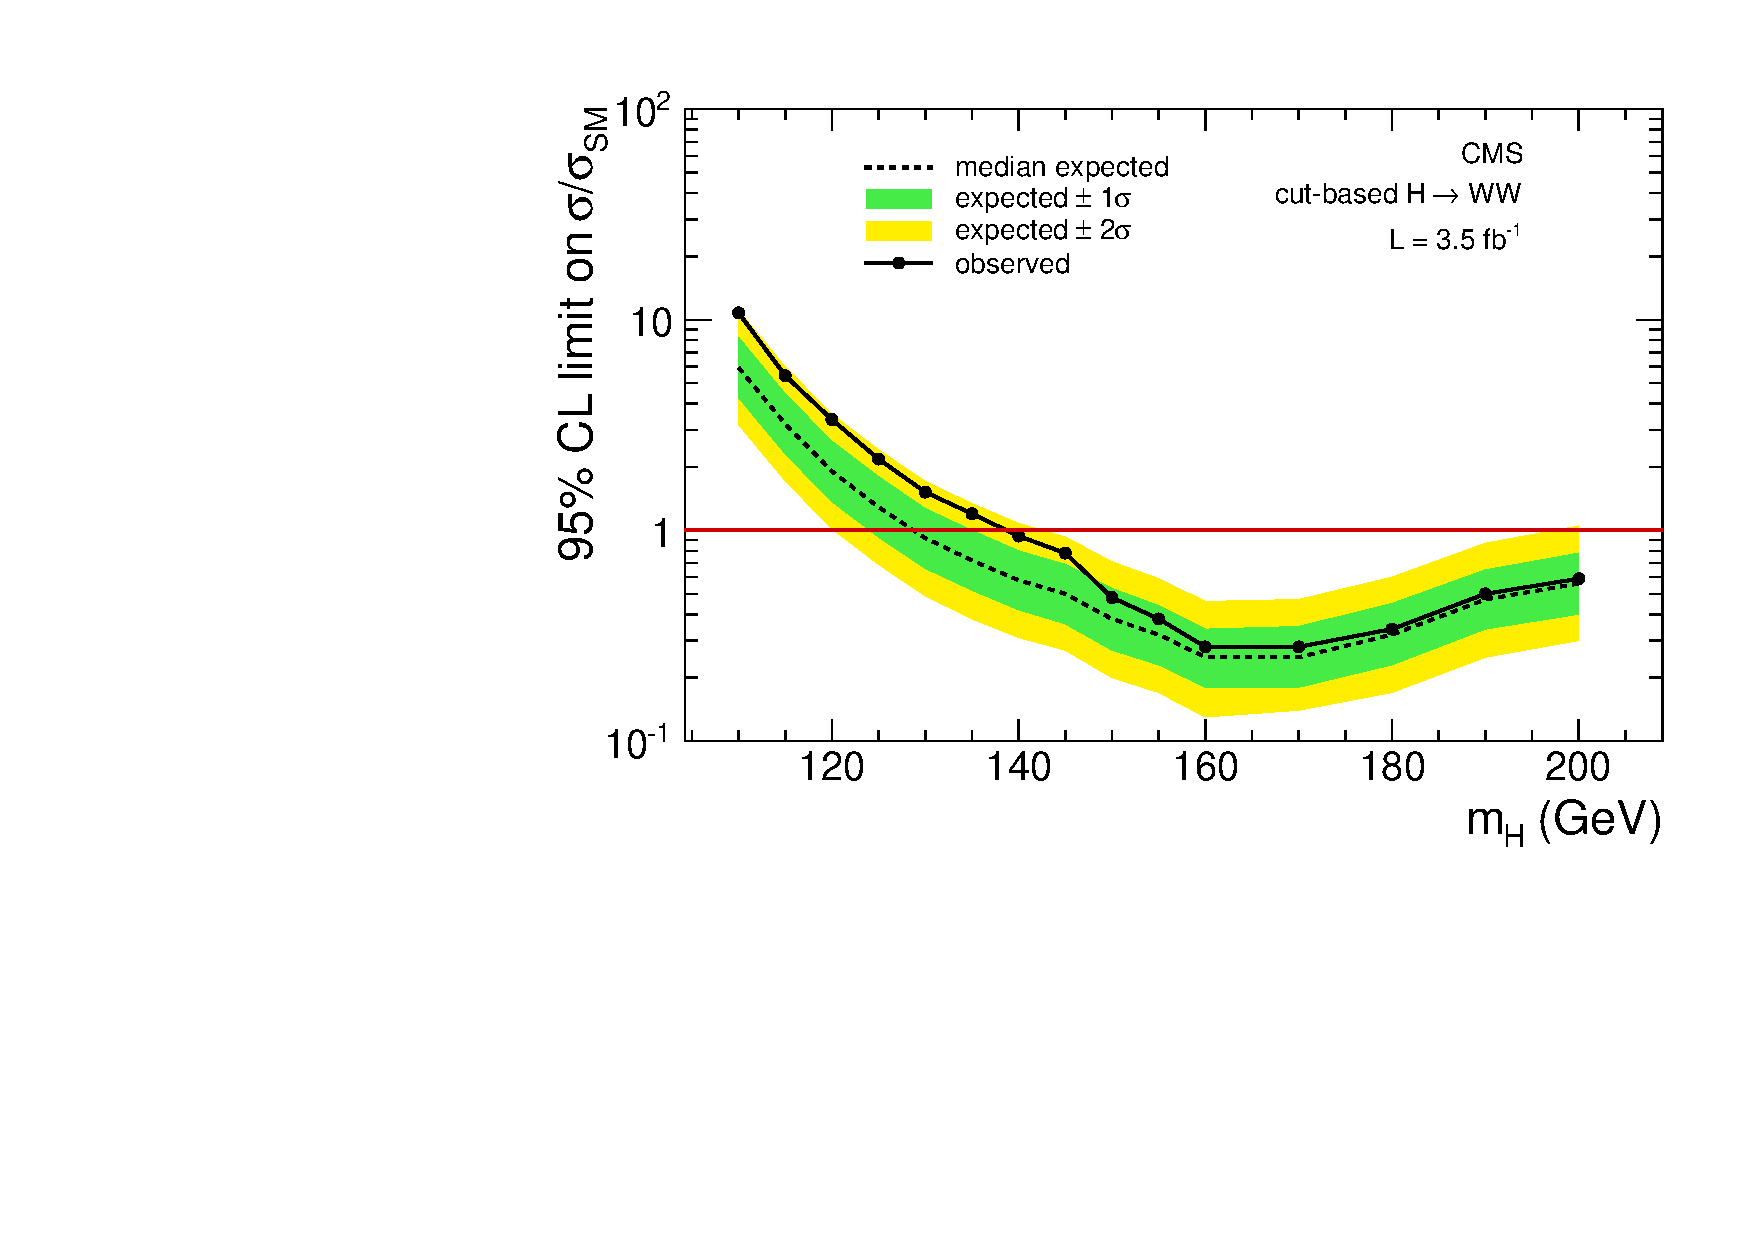
\includegraphics[width=.45\textwidth]{figures/limits_nj_ICHEP_MH125_cut_8TeV.pdf}
}
\centering
\subfigure[shape-based]{
\centering
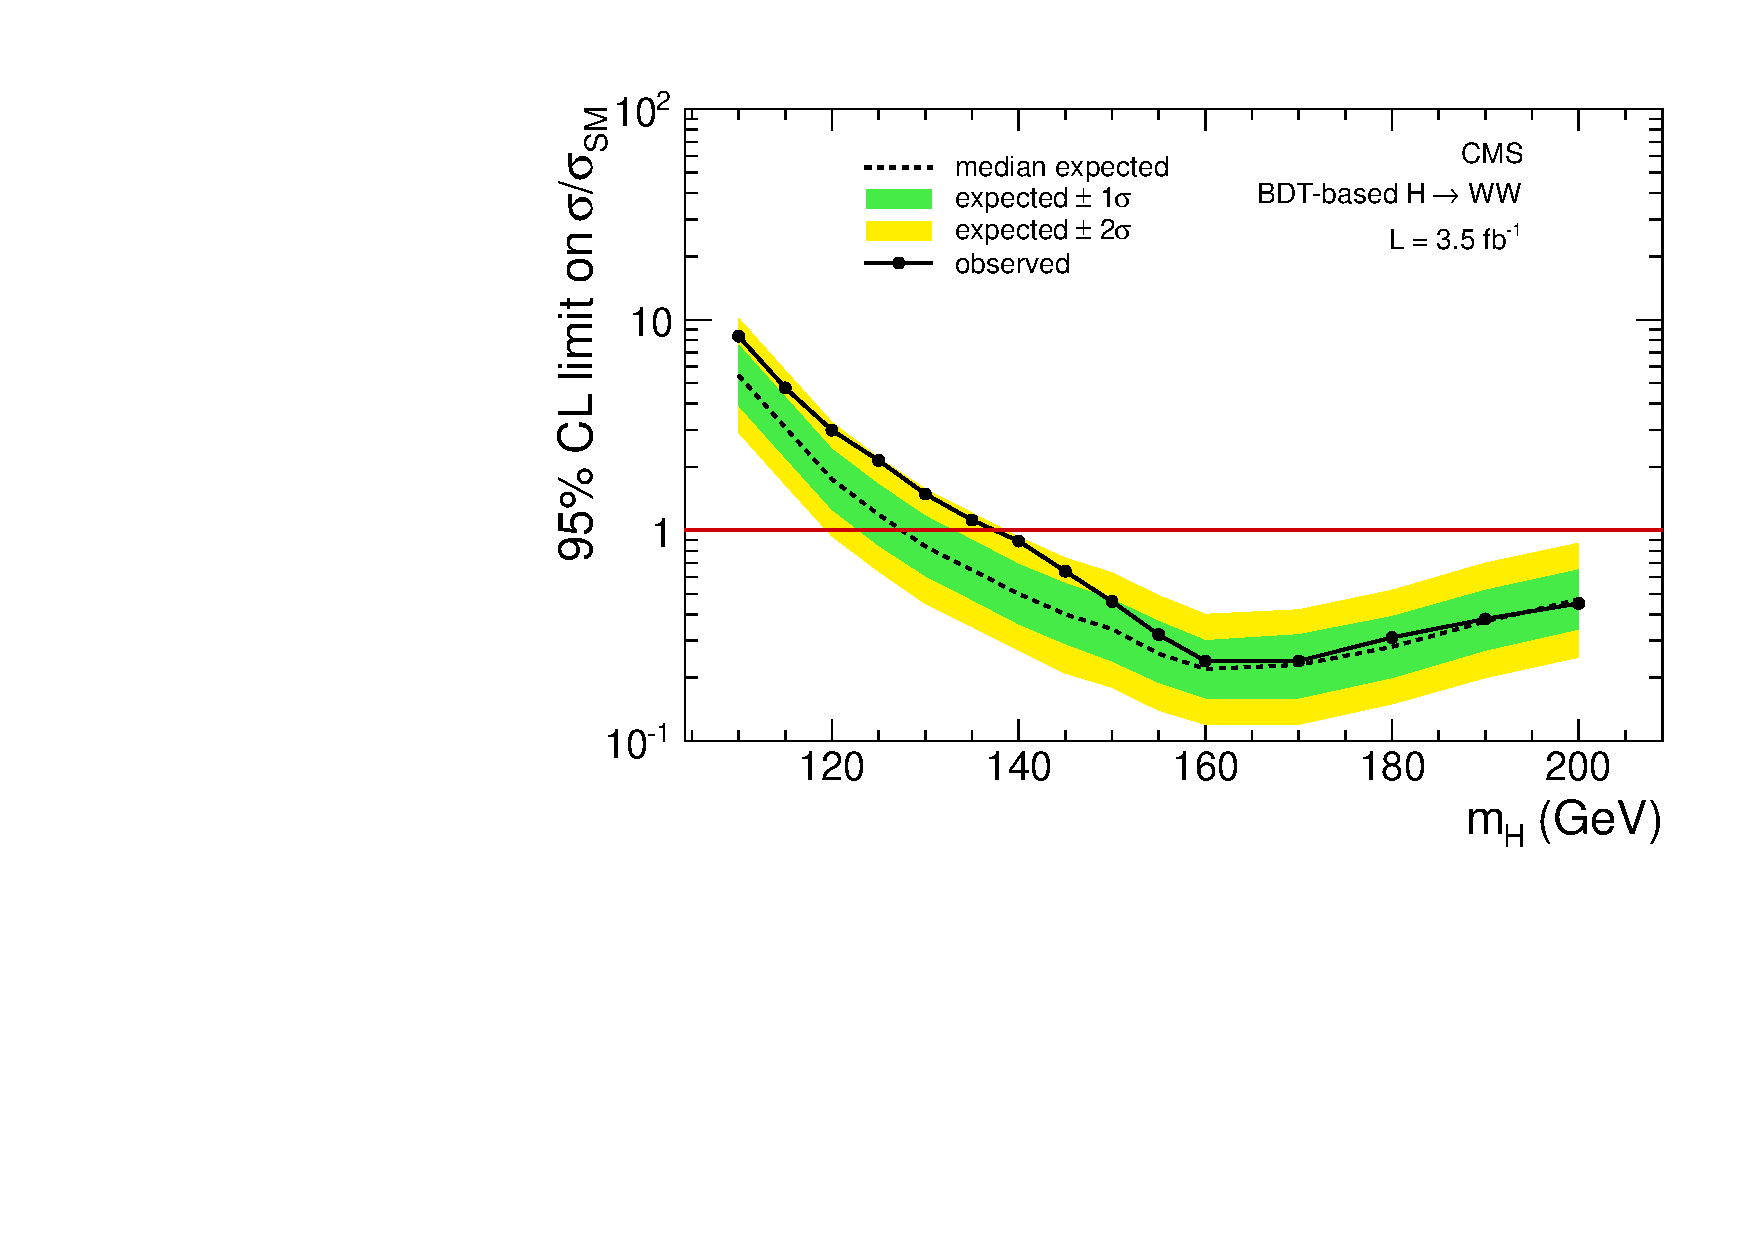
\includegraphics[width=.45\textwidth]{figures/limits_nj_ICHEP_MH125_shape_8TeV.pdf}
}
\caption{Upper limits in the 0/1/2-jet bins for SM Higgs using the
  {\bf shape-based} $\mll$ analysis with 3.5$\ifb$ of data in the case of the
  presence of a Higgs with $\mHi = 125~\GeV$.}
\label{fig:uls_mh125_nj}
\end{figure}
%%%%%%%%%%%%%%%%%%%%%%%%%%%%%%
